\begin{figure}
\vspace{-1cm}
\centering
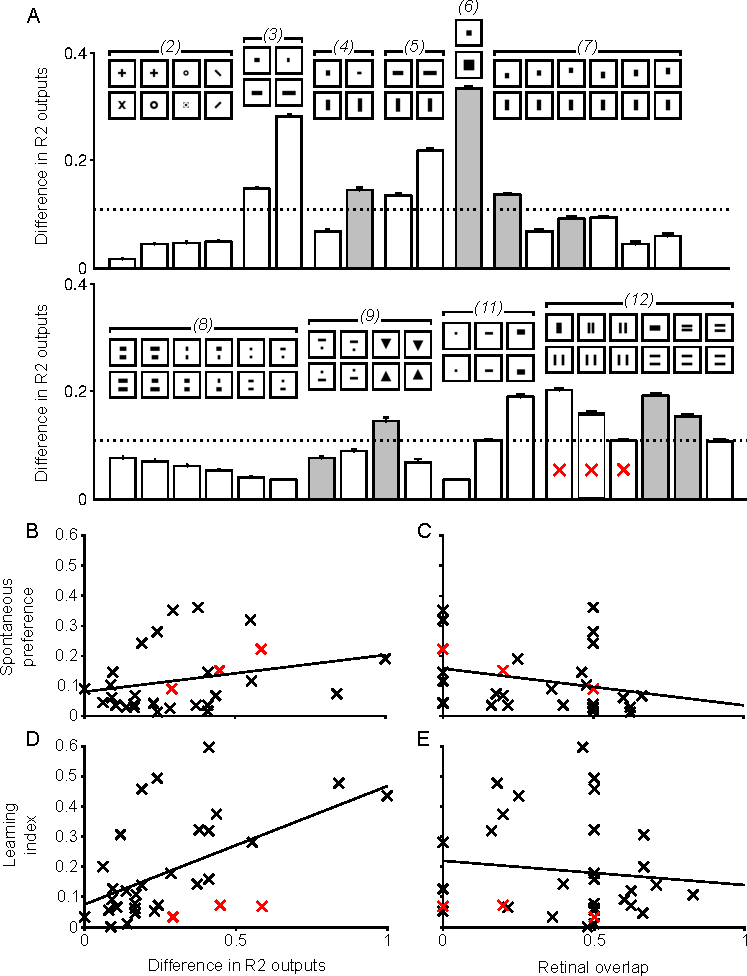
\includegraphics{figures/pattern}
\caption{[NB: I haven't put in the pattern pairs yet, but this should give an idea of the layout.]
Outputs of simulated R2 cells for published pattern pairs. Whether a pattern pair is discriminable by flies can be predicted partly on the basis of the difference in R2 activity.
The patterns tested here are drawn from \protect\cite{Ernst1999} and are grouped together according to the figures in which they appear in that work.
The corresponding figure numbers are shown in parentheses.
All patterns for which the significance of `learning preference' ($\overline{\mathrm{DCP}}$) was given are included.
Grey bars indicate that the $\overline{\mathrm{DCP}}$ for the pattern was significant ($p<.05$).
A higher score indicates a greater \ac{rms} difference in R2 activity and thus that the pattern was more discriminable by the simulation.
In general, within these groups, the patterns where there was a significant learned preference (in \protect\cite{Ernst1999}) have a greater difference in activity.
Performance on more `horizontal' patterns (e.g. \emph{(3)} and the final three patterns in \emph{(12)}) was poor in the behavioural experiments, but better in simulation.
This is perhaps due to the horizontal motion of the patterns in training, as noted in \protect\cite{Ernst1999}.
At the bottom are shown scatter plots of R2 difference (the `RF Model') and retinal overlap (the `Retinotopic Model') \emph{vs} learning index ($\overline{\mathrm{DCP}}$) shown in Ernst and Heisenberg \protect\cite{Ernst1999}.
The correlation for the RF Model was found to be significant (Spearman's rank, $n=34, \rho=.615, p<.005$), but not for the Retinotopic Model ($n=34, \rho= -0.215, p=\mathrm{n.s.}$).
}
\label{fig:pattern}
\end{figure}
